%TODO: Vikram, figure is missing
%TODO: Figure out if we can publicly share a sanitized version of the MAC instruction's timing reports
%TODO: Reconfig. in LRU? Maybe this is not even required ...
%TODO: Ensure merge strategy for bounded packet history is available in the TR
%TODO: Prove convergence of fixed point algorithm

\chapter{Understanding mergeability}

\section{The problem}

A programmer supplies an aggregation function $f$. $f$ takes as inputs an n-bit \emph{state}
vector and a p-bit \emph{packet header} vector and returns an updated $n$-bit
\emph{state} vector. $f$ captures incremental computations over packet streams,
such as a count of packets or an exponentially weighted moving average of
packet latencies. $f$ can only represent incremental computations where the
size of state is fixed and doesn't grow with the length of the packet stream.
For example, $f$ can't represent a median over the packet stream.

Given $f$, we want two implementation functions: an incremental function implementation $g$
 and merge function implementation $m$ that can merge results from
running $f$ over separate packet streams. Specifically, can we merge
two results from running $f$ on two packet streams into one result,
equivalent to running $f$ on the concatenated stream? Formally, we suppose that the state used by
the implementation is $n' \geq n$ bits. The paper refers to the merge function using $a$ auxiliary bits.
Here, $a = n' - n$. 

\begin{align}
f : \{0, 1\}^n \times \{0, 1\}^p & \rightarrow \{0, 1\}^n \mbox{(programmer's incremental computation)} \nonumber \\
g : \{0, 1\}^{n'} \times \{0, 1\}^p  & \rightarrow \{0, 1\}^{n'} \mbox{(implementation's incremental computation)} \nonumber \\
m : \{0, 1\}^{n'} \times \{0, 1\}^{n'} & \rightarrow \{0, 1\}^{n'} \mbox{(implementation's merge operation)} \nonumber \\
h : \{0, 1\}^{n'}               & \rightarrow \{0, 1\}^n  \mbox{(transform
 implementation state to programmer state)} \nonumber \\
s_0  & \in \{0, 1\}^n \mbox{(programmer's start state)} \nonumber \\
s'_0 & \in \{0, 1\}^{n'} \mbox{(implementation's start state)} \nonumber \\
m(s'_0, s') & = s' \ \ \forall s \in \{0, 1\}^{n} \mbox{($s'_0$ is an identity for $m$)} \nonumber \\
(g, m, h, s'_0) & \mbox { merges } (f, s_0) \mbox{ if} \nonumber \\
s_0 & = h(s'_0) \mbox{(implementation's start matches with programmer's start)} \label{eqn:start_condition} \\
f(f(f(s_0, P_1), P_2), \dots, P_n) & = h(g(g(g(s'_0, P_1), P_2), \dots, P_n)) \ \forall n \in \mathbb{N} \ \ P_1, P_2, \dots, P_n \in \{0, 1\}^p \label{eqn:projection_condition} \\
h(g(g(g(s'_0, P_1), P_2), \dots, P_{i+j})) & =h( m(g(g(g(s'_0, P_1), P_2), \dots, P_{i}), \nonumber \\
&\ \ \ \ g(g(g(s'_0, P_{i+1}), P_{i+2}), \dots, P_{i+j}))) \nonumber \\
\forall i, j \in \mathbb{N} & \ \  P_1, P_2, \dots, P_{i+j} \in \{0, 1\}^p \label{eqn:merge_condition}
\end{align}

Here $f, g, m,$ and $h$ are assumed to be efficiently computable functions. We use the notation $f(s, \{p_1, \ldots p_k\})$ to denote the composition of $f$ over a sequence
of packets, similar to a fold function. Additionally, we say that a merge function successfully merges an aggregation function if Equation~\ref{eqn:merge_condition} holds. 

\section{The Merge Procedure}

For queries that are linear in state, the state update takes the form $\mathbf{S} = A(\mathbf{p})\cdot\mathbf{S} + B(\mathbf{p})$, where $S$ is a vector of state, and $A$ and $B$ are functions of the previous $k$ packets (denoted by $\mathbf{p})$. Here $k$ is an arbitrary integer.

\subsection{Single packet history}

Consider the case where $k = 1$. If the state is $\mathbf{S}$ at any point in time, then after $N$ packets,
$\mathbf{S_N} = A^N\cdot \mathbf{S} + $ terms independent of $S$. Here, $A^N$ is shorthand for $A(p_N)\cdot A(p_{N-1}) \cdot \ldots \cdot A(p_1)$
Therefore to merge an evicted value $\mathbf{S_N}$ with the existing value $\mathbf{S}_{backing}$ in the backing store,
we need to replace $\mathbf{S}$ with $\mathbf{S}_backing$ in the expression for $\mathbf{S_N}$ by computing:
\[ \mathbf{S_N} - A^N \cdot \mathbf{S} + A^N \cdot \mathbf{S}_{backing} = \mathbf{S_N} + A^N(\mathbf{S}_{backing} - \mathbf{S}) \]
The merge procedure is straightforward: the switch keeps $A^N$ as auxiliary state and passes it with $\mathbf{S_N}$ to the backing store to complete the merge.
The backing store already knows $S$, since it is the default starting value for the state, which does not change.

\subsection{Bounded packet history}

The required auxiliary state is more complex for larger values of $k$. If $k = 1$, $A(p)$ and $B(p)$ are known to the switch for every packet. However, for larger values of $k$, the switch needs access to older packet fields to compute $A(\mathbf{p})$ and $B(\mathbf{p})$. This means the values of $A$ and $B$ are themselves incorrect for the first $k-1$ packets after an eviction, an issue that must be addressed by the merge procedure.

Consider Figure~\ref{fig:bph-merge} for $k = 3$. Once the switch performs an eviction at $T_1$,
the switch cannot properly update the its state for the next two packets (first packets of the subsequent epoch).
It thus starts updating its state from the third packet onwards and entrusts the backing store to
fill the ``hole'' caused by missing the first two state updates.

\begin{figure}[h]
\centering
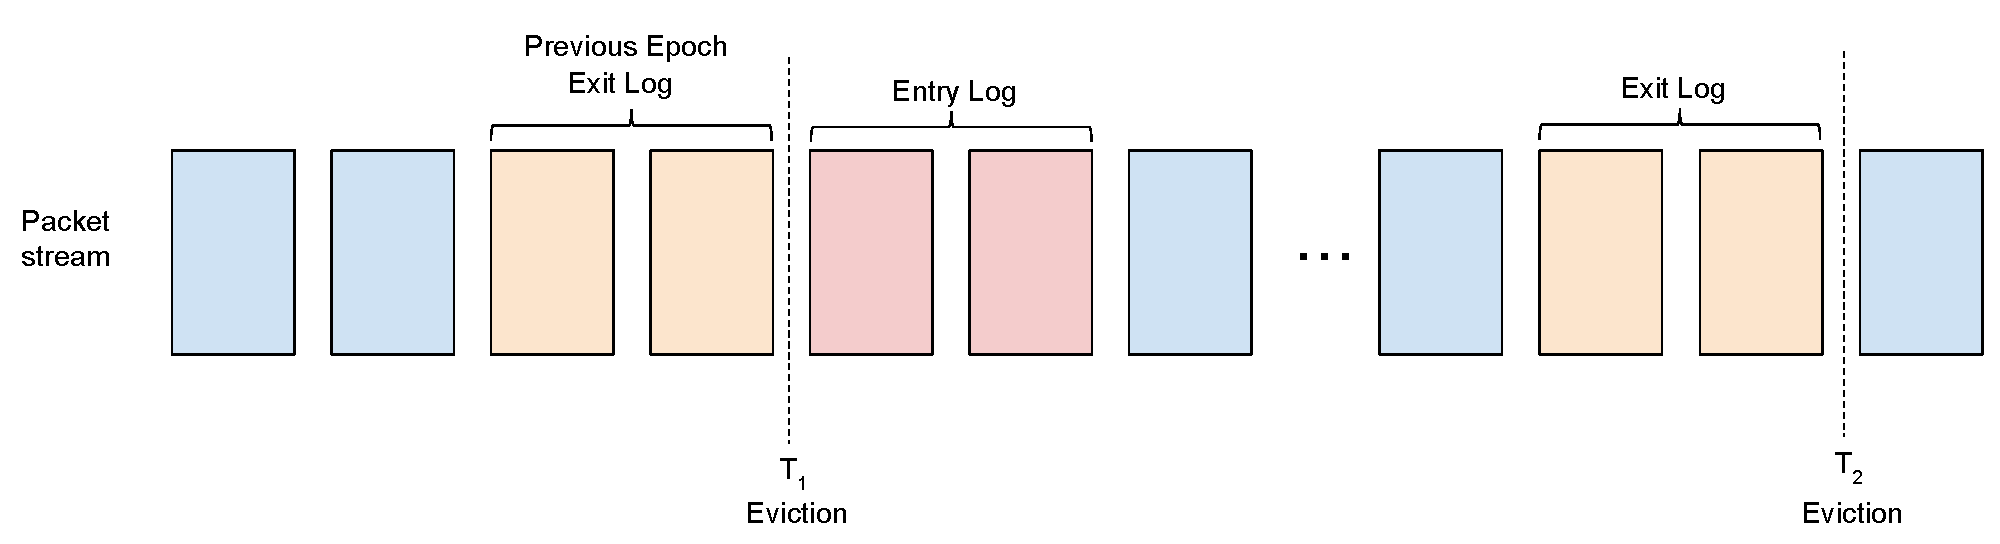
\includegraphics[width=0.7\linewidth]{pq_merge_tr_bph.pdf}
\caption{Entry and exit log for an eviction, with $k = 3$.}
\label{fig:bph-merge}
\end{figure}

To perform the merge successfully,
the backing
store needs two additions pieces of information, 
in addition to the query-specific state $A^N$ discussed in the previous section:
\begin{itemize}
\item The last $k-1$ packets from the \emph{previous epoch}, called the \emph{exit log} $R$ of the previous epoch.
\item The first $k-1$ packets from the \emph{current epoch}, called the \emph{entry log} $X$ of the current epoch. 
\end{itemize}

Upon merging, the backing store receives $S$, $R$, and $X$, and must merge them with $S_{backing}$. First, the backing store runs the actual aggregation function over $R$ starting from $S_{backing}$: $S' = g(S_{backing}, R)$. Doing this requires the backing store to use the exit log of the \emph{previous} epoch. The backing store then performs a standard merge
 $S'' = m(S', S)$ and stores $X$ for use in the \emph{next} epoch's merge.

\section{The Closure Graph}

Before proceeding with the proofs, we introduce the directed \emph{closure graph} of $f$, denoted $G(f)$. Suppose that at some point during the aggregation, 
the programmer specified state is $s$. After running through some additional packets, that state is updated to $s'$. If $s$ is known, then computing
$s'$ is straightforward: simply execute the aggregation $f$ on all the packets seen in the interim. However, if $s$ is \emph{not} known, we can instead
use the packets seen to compute a function that tells us how to get from \emph{any} state $s$ to the final desired state $s'$. That is, given a sequence of packets $\{p_k\}$,
we can compute an \emph{iterated} function $f_i \in \{0,1\}^n \rightarrow \{0,1\}^n$, such that for any state $s$, $f_i(s) = f(s, \{p_k\})$. For an empty sequence, the corresponding iterated function is the identity.
Our goal is to store some compact representation of the iterated function in the on-chip cache. This iterated function is updated with each new packet that is seen, so that when a key is evicted from the on-chip cache,
an identifier for the updated iterated function is sent to the backing store. The backing store then applies this iterated function to the state $s_{backing}$ stored from a previous eviction to get the new value.

How does one update the iterated function stored on the switch? The vertices of the closure graph of $f$ are iterated functions $f_i$, and we let $|G(f)|$ indicate the number of vertices. Since there are a finite number of functions $\{0, 1\}^n \rightarrow \{0, 1\}^n$, the size of the graph is bounded.
Each vertex has an outgoing edge corresponding to every possible packet. For a given packet $p$, the iterated function $f_i$ has an edge to the function $f_j$ satisfying $f(f_i(s), p) = f_j(s)$ for all $s$.
The closure graph thus has the following property: given a sequence of packets $\{p_1, \ldots p_k\}$, start at the identity function and, on the $i$th step, follow the edge corresponding to each packet $p_i$. The ending vertex of this process is the iterated function that captures the effect of this packet sequence on any starting state. We say that this ending vertex is the result of \emph{updating the iterated function} by the given sequence of packets. To update the iterated function stored on the switch given a new packet, simply follow the edge labeled with that packet.

\begin{theorem}[Publication Theorem 3.1]
A merge function exists to successfully merge an aggregation function $f$, providing it can use up to $n2^n$ auxiliary bits.
\end{theorem}
\begin{proof}
We can represent each iterated function $f_i$ in $n2^n$ bits, using a list of $2^n$ $n-$bit numbers, where the $k$th item is $f_i(k)$. The switch stores this representation. For each new packet $p$, the switch computes the update to each number in the list: $f_i(k) \rightarrow f(f_i(k), p)$. Upon a merge, the switch sends this representation to the backing store, which can then evaluate $f_i(s_{backing})$, where $s_{backing}$ is the value stored in the backing store.
\end{proof}

Note that the switch needs to tell the backing store what update to perform on the value it currently has. Each iterated function in the closure graph is a possible update, so the switch needs to convey at least $\log |G(f)|$ auxiliary bits for the merge to be possible.

As an example, consider a simple counter, where $f(s, p) = s + 1$ and $s_0 = 0$. If the counter has $n$ bits, the closure graph is a ring of size $2^n$, where the $i$th vertex encodes the iterated function $f_i(s) = s + i$. Note that all edges from the $i$th vertex point to the $i+1$st vertex. For every observed packet, the switch walks one step further around the ring. This is implemented efficiently via adding 1 to an $n$-bit counter. Upon merging after $K$ packets, the iterated function on the switch is $f_{k}$, where $k = K \mod 2^n$. Upon merging, this is sent to the backing store, which then knows to add $k$ to the existing backing store value.

In general, requiring $n2^n$ bits is typically infeasible for even moderate values of $n$. This is where the linear-in-state and associative conditions come in. We show that either of these conditions is enough to require only $O(n)$ auxiliary bits of space.

\begin{theorem}[Publication Theorem 3.2]
 Aggregation functions that are either linear-in-state or associative have a merge function that uses only $O(n)$ auxiliary bits.
\end{theorem}
\begin{proof}
The associative condition is trivial: by definition, no auxiliary bits are required. 
Suppose $f$ is an aggregation function that is linear in state, i.e. $f(\mathbf{S}, p) = \mathbf{A}(p) \cdot \mathbf{S} + \mathbf{B}(p)$, where $\mathbf{S}$ is a state vector, and $\mathbf{A,B}$ are matrices depending only on the incoming packet. Then:
\[ f(\mathbf{S}_0, \{p_1, \ldots, p_k\}) = \mathbf{A}(p_k)\ldots \mathbf{A}(p_1) \cdot \mathbf{S}_0 + \mathbf{C}(p_1, p_2, \ldots, p_k) \equiv \mathbf{A'} \cdot \mathbf{S}_0 + \mathbf{C}(p_1, \ldots, p_k)\]
where $\mathbf{C}$ is some function of only the packets and $\mathbf{A'}$ is a composition of the $\mathbf{A}$ matrices for the observed packets. The switch keeps track of $\mathbf{A'}$ and $\mathbf{C}$, which requires $O(nd^2)$ space where $d$ is the number of pieces of state, each of which we assume has size $n$. These matrices are sent to the backing store upon eviction, at which point the merge operation computes the new backing store value:
\[ \mathbf{S}_d \leftarrow \mathbf{C}(p_1, \ldots, p_k) + \mathbf{A'} \cdot \mathbf{S}_d \]
It's easy to verify that this is the proper merge procedure.
\end{proof}

However, there are some functions that are not mergeable with so few auxiliary bits. Take the following TCP-non-monotonic function:
\begin{verbatim}
def nonmt(maxseq, count, tcpseq):
  if maxseq > tcpseq:
    count = count + 1
  else:
    maxseq = tcpseq
  nm_q = groupby(pktstream, 5tuple, nonmt);
\end{verbatim}

\begin{theorem}[Publication Theorem 3.3]
The TCP-non-monotonic function requires at least $n2^n$ auxiliary bits to merge.
\end{theorem}
\begin{proof}
Two pieces of state must be stored: the max sequence number and the count. For simplicity, we assume each piece of state requires $n$ bits.
We present a family of packet sequences, such that there is an injection between the sequences and vertices in the closure graph of $f$. In other words, starting from the identity, updating the identity iterated function by each sequence in this family will result in a distinct iterated function. 

Consider a family of packet sequences parameterized by a tuple $(a_0, a_1, \ldots a_{2^n-1})$: the sequence consists of $a_i$ packets with sequence number $i$, in increasing order of $i$. For each such tuple, performing an update $U$ of the identity iterated function by the sequence for that tuple results in the following final iterated function:
\[ U(a_0, \ldots, a_{2^n-1}) = f\quad\quad \text{such that} \quad\quad f(x,y) = \left(2^n - 1, (y + \sum_{i=0}^{x-1} a_i) \mod 2^n\right) \]
where $x$ and $y$ are the max sequence number and count, respectively. To see why this is the case, recall that the iterated function is taking some \emph{previous} max seq. number and count and trying to update it by the packet sequence. If the max sequence number was $x = k$ before, then the count will increase by the number of packets with sequence number $< k$, which is $\sum_0^{k-1} a_i$.
\begin{lemma}
$U$ is an injection.
\end{lemma}
\begin{proof}
If $(a_0, \ldots, a_{2^n-1}) \neq (a_0', \ldots, a_{2^n-1}')$, then there is some $k$ such that $a_k \neq a_k'$ but $a_j = a_j'$ for all $j < k$. Note: $k= 0$ may satisfy this condition. Let $U(a_0, \ldots, a_{2^n-1}) = f$ and $U(a_0', \ldots, a_{2^n-1}') = f'$. Then, for any $y$:
\[ f(k+1, y) - f'(k+1,y) = \left(0, \sum_{i = 0}^k a_i - \sum_{i = 0}^k a_i'\right) = (0, a_k - a_k') \neq (0, 0) \]
so $f \neq f'$, making $U$ an injection.
\end{proof}
There are $2^{n2^n}$ such packet sequences, meaning that the closure graph has at least $2^{n2^n}$ distinct vertices, and thus number of auxiliary bits needed is at least $\log 2^{n2^n} = n2^n$. 
\end{proof}

Now we turn to the question: given an aggregation function, how easy is it to compute a merge function that uses the minimal number of auxiliary bits?
Since we know that the minimal number of bits is $\log |G(f)|$, we can construct $G(f)$. This approach is extremely inefficient, but it works. 

\begin{theorem}
Given an aggregation function $f$, an algorithm exists to compute a merge function using the minimal number of auxiliary bits.
\end{theorem}
\begin{proof}
To construct the closure graph, we start with a single node representing the
identity function. Starting at this node $f_0$, we enumerate all $p$-bit values for a
single packet $P$, and compute the updated iterated function $f_P$ satisfying $f_P(s) = f(f_0(s), P)$ for all $s$.
If this iterated function has not been seen yet, we create a new node for it.
We join two nodes by an edge labeled
with the packet value that causes the transition between those two nodes and
repeat this process from each newly created node until all edges out of a node
lead back to existing nodes\footnote{We need a way to check node equality,
i.e., function equality. We do this by a brute force check on all inputs to
both nodes/functions.}.

There are $2^{n2^n}$ possible iterated functions. We assume that given an iterated function,
it is possible to find that function in the existing partial closure graph in time $O(n2^n)$,
the number of bits needed to represent the number of iterated functions in the worst case.
Then, since we must enumerate every possible $p$-bit packet the total runtime is:
\[ O(\text{\# iters} \cdot \text{\# packets} \cdot \text{\# time to test if function has been seen}) =  O\left(2^{n2^n} \cdot 2^p \cdot n2^n\right) \]
\end{proof}

This algorithm is intractable in practice. However, a polynomial time algorithm is also likely intractable.
We demonstrate this hardness result by considering a decision version of this problem:
given an aggregation function $f$ and merge function $m$, does $m$ successfully merge $f$ for all possible packet inputs?
This problem turns out to be co-NP-hard.

Before we launch into the hardness proof, we must limit the scope of the problem. ``All possible packet inputs'' includes
packet sequences of arbitrary length. However, we can restrict ourselves to sequences up to $2^n$ packets.

\begin{theorem}
To determine whether $m$ merges $f$ on every packet sequence, it is sufficient to consider packet sequence up to
length $2^n$.
\end{theorem}
\begin{proof}
We show it is sufficient to check equation~\ref{eqn:projection_condition} on
packet streams of length $L <= M = 2^{max(n, n')}$. This check fails only if
there is a stream $P_{false}$ of length $L > M$ that falsifies
equation~\ref{eqn:projection_condition}. However, there must then also be a
smaller stream $P_{small}$ of length $L'<=M$ that falsifies
equation~\ref{eqn:projection_condition}.

To see why, let's say packet $A$ within $P_{false}$ first falsifies
equation~\ref{eqn:projection_condition}. If $A's$ position within $P_{false}$
is less than or equal to $M$, the substream up to and including $A$ is
$P_{small}$. If not, running $f$ repeatedly on the substream of packets until
$A$ will result in some state value $s$ being repeated twice, after seeing
(say) packets $P_{1}$ and $P_{2}$. We can remove all packets after $P_{1}$ and
before $P_{2}$, creating a shorter stream that still
falsifies~\ref{eqn:projection_condition}.  This process can be repeated until
the stream length is less than or equal to $M$. This will eventually happen
because there will always be a repeated state value by the pigeon-hole
principle because the number of packets in a stream is greater than the number
of distinct states.
\end{proof}

Now we know that checking whether $m$ successfully merges $f$ is actually possible.
However, it is likely intractable. We'll show this by showing that it is hard to perform the
 simple action of \emph{verifying}
that a \emph{given} merge function successfully merges a given aggregation function.

\begin{theorem}[Publication Theorem 3.4]
Given a merge function $m$ and aggregation function $f$, verifying that $m$ successfully
merges $f$ is co-NP hard.\footnote{co-NP is made up of problems
that are complements of problems in NP.}
\end{theorem}
\begin{proof}
We'll show that $MERGE$ is co-NP-hard by reducing $TAUTOLOGY$ (a known
co-NP-complete problem) to $MERGE$.

An instance of $TAUTOLOGY$ is a function $t$. The output is 1 when $t$ is a
tautology, 0 otherwise. $TAUTOLOGY(t)$ can be reduced to\footnote{This is a
polynomial many-to-one reduction or a Karp reduction.} $MERGE(s \oplus t', 0, s
\oplus t', OR, I, 0)$,\footnote{t'(P) = (NOT t(P))}where
\begin{enumerate}
\item $s \in \{0, 1\}$
\item $t : \{0, 1\}^p \rightarrow \{0, 1\}$
\item $OR$ is the boolean OR function on two bools.
\item $I$ is the identity function.
\end{enumerate}

First, we observe that $MERGE(s \oplus t', 0, s \oplus t', OR, I, 0)$ decides whether statement~\ref{eqn:merge} is true:
\begin{align}
t'(P_1) \oplus t'(P_2) \oplus \dots t'(P_{i+j}) & = (t'(P_1) \oplus t'(P_2) \dots t'(P_{i})) OR (t'(P_{i+1}) \oplus t'(P_{i+2}) \dots t'(P_{i+j})) \label{eqn:merge} \\
\forall i, j \in \mathbb{N} \ \ & P_1, P_2, \dots, P_{i+j} \in \{0, 1\}^p \nonumber
\end{align}

Next, we prove a lemma that shows the reduction from $TAUTOLOGY$ to $MERGE$.

\begin{lemma}
Statement~\ref{eqn:merge} is true iff $t'(P) = 0 \ \forall P$.
\end{lemma}
\begin{proof}
Let's suppose $t'(P) = 0 \ \forall P$. It is easy to see that statement~\ref{eqn:merge} reduces to 0 on both the LHS and RHS. If on the other hand, $t'(P^*) = 1$ for some $P^*$. Then, we set:
\begin{enumerate}
\item $i = 1$
\item $j = 2k - 1$
\item $P_1 = P_2 = \dots = P_{i+j} = P^*$
\end{enumerate}
The LHS is an XOR over an even number of 1s, which is 0. The RHS is an OR of 1
and something else, which is 1. So, we have found one setting of the quantified
variables that falsifies statement~\ref{eqn:merge}.
\vspace{\baselineskip}
\end{proof}

It is straightforward to see how $TAUTOLOGY(t(P))$
reduces to $MERGE(s \oplus t', 0, s \oplus t', OR, I, 0)$, showing that $MERGE$
is co-NP-hard.
\end{proof}

\end{document}
